\subsection{Dancing Experiment}
Using the PAGI World environment, we set out to create an artificial intelligence agent that is capable of learning through reinforcement provided by a human teacher.  PAGI World allows the user to send commands to the agent via a small input box.  We used this feature to teach the agent how to perform a specific dance routine in an extremely brief training period.

The agent entered the world with little prior knowledge.  In fact, throughout the learning period, the amount of information known by the agent remained relatively constant.  The agent initially knew how to perform several dance moves, e.g.: a slide from one side to another, a jump with a 360-degree spin, and a dance move commonly referred to as `raising the roof.'  Additionally, the agent had a two-dimensional table of dance moves.  This move table, described in detail below, is intended to represent the agent's knowledge of how to combine the moves it knows, in order to perform dance routines.  The agent starts out with no real understanding of how to perform a cohesive dance, but through interaction with the user, the agent can learn any routine.


%INSERT MOVES
\begin{figure}[h]
	\centering
	\begin{subfigure}{.5\textwidth}
		\centering
		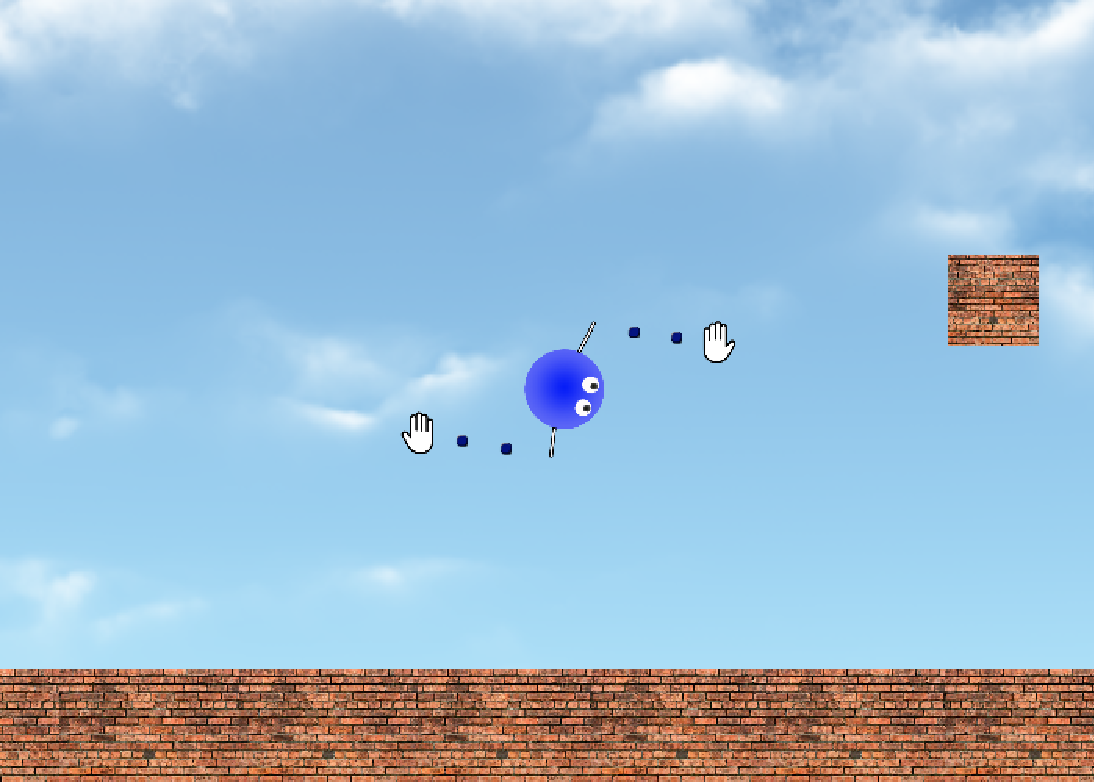
\includegraphics[width=.8\linewidth]{360cropped}
		\caption{Agent performing a Jump 360}
		\label{fig:sub1}
	\end{subfigure}%
	\begin{subfigure}{.5\textwidth}
		\centering
		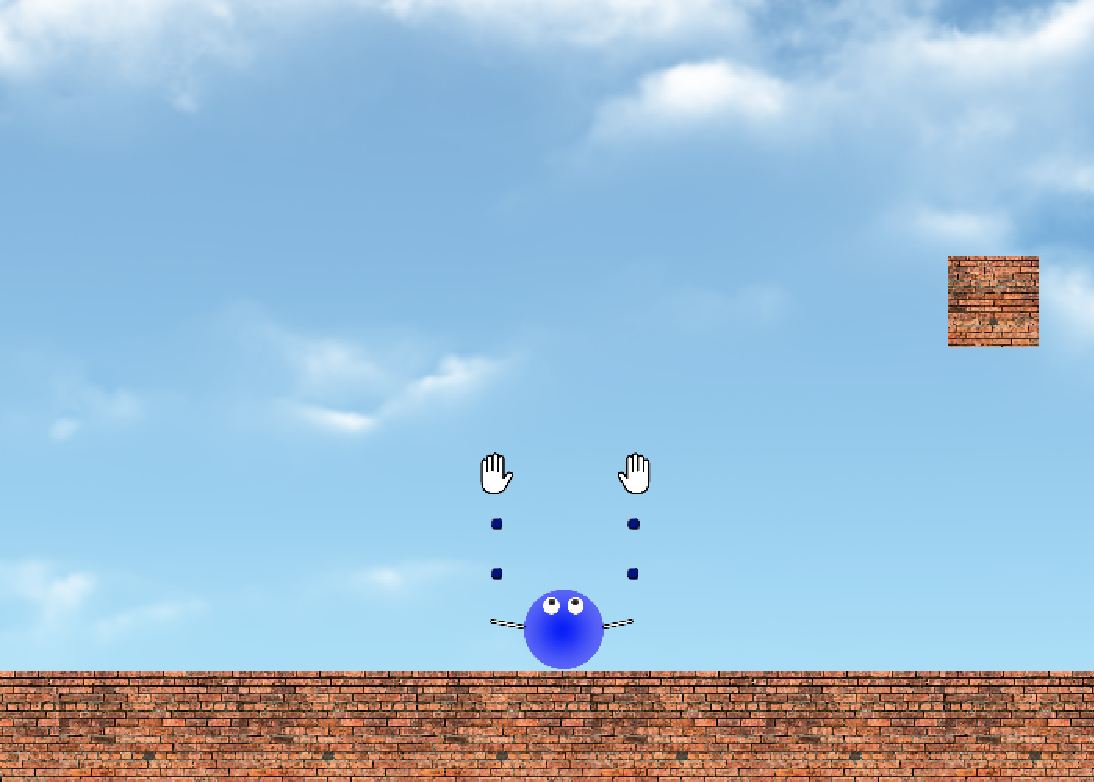
\includegraphics[width=.8\linewidth]{roofcropped}
		\caption{Agent 'raising the roof'}
		\label{fig:sub2}
	\end{subfigure}
	\caption {Agents performing pre-known dance moves}
	\label{fig:dances}
\end{figure}


Table \ref{unlearn} refers to an initial move table.  The top row denotes the current state of the agent, determined by which move the agent performed previously.  The `begin' column indicates the probability that a particular move being the first move of the sequence.  As you can see, the initial probability for any move to be selected as the first dance move is 0.25.  If, for example, move 3 was chosen to be the first move, the agent would then look under the move 3 column to select the next move.  Again, all these probabilities are equal, so the next move will be chosen at random.  The move selection process would continue in this fashion, until the dance to be performed is the correct length.

%INSERT TABLE 1 HERE
\begin{table}[h]
	\begin{center}
		\begin{tabular}{| c | c | c | c | c | c |}
		
		\hline
			 & begin & move 1 & move 2 & move 3 & move 4 \\	\hline	
			move 1 & 0.25 & 0.25 & 0.25 & 0.25 & 0.25 \\	\hline
			move 2 & 0.25 & 0.25 & 0.25 & 0.25 & 0.25 \\	\hline
			move 3 & 0.25 & 0.25 & 0.25 & 0.25 & 0.25 \\	\hline
			move 4 & 0.25 & 0.25 & 0.25 & 0.25 & 0.25 \\	 \hline
		
		\end{tabular} %
	\end{center}
	\caption {Example unlearned move table}
	\label{unlearn}
\end{table}
In order to get the agent to learn a dance, we used a first-order Markov chain.  This allowed the agent to remain essentially memory-less, as `first-order'�� implies that the agent'��s next action is based solely on its current state,�� or in our case, the move that came immediately before.  This could easily be extended to a higher order for more complicated dances or for other desired goals.

If you asked the agent to perform a 4-move dance initially, moves would be selected at random, as each move has an equal probability to be chosen regardless of what state the agent is in.  In order to begin teaching the agent, the user must tell the agent to enter learning mode. Learning mode begins with the agent generating all possible moves for all possible states, using iterative deepening depth first search.  The first moves in this sequence would be single moves; these are used to 'teach' the first move in the desired dance.  After these single moves, the agent would move on to two-move combinations.  The agent would perform a move from the tree, then await feedback from the user.  The user would respond with either `good' or `bad' using the text box built in to PAGI World.  The agent would store this feedback, and then continue on to the next move in the tree.  After the agent received feedback from all possible single moves/move combinations, the agent would begin to generate the new move table.  Each move for a particular state would receive a probability of $1/N$, where $N$ is the number of moves in that state that received positive feedback.  This table would then replace the move table previously in the agent's knowledge.

Table \ref{tab:learn1} demonstrates what the move table could look like after learning has occurred.  As before, the top row indicates the current state of the agent, and the probabilities a move will be chosen for a particular state corresponds to the row labeled accordingly.  In this table, move 2 is the only move that has a chance to be picked as the first move.  From there, the agent will move on to the `move 2' state to select the next move.  In this state, the only move that can be chosen is move 3.  The agent will continue selecting moves in this fashion, until the dance is of the correct length, in this case, a 4 move dance.

%INSERT TABLE 2 HERE
\begin{table}[h]
	\begin{center}
		\begin{tabular}{| c | c | c | c | c | c |}
		
			\hline
			 & begin & move 1 & move 2 & move 3 & move 4 \\	\hline	
			move 1 & 0 & 0 & 0 & 0 & 0 \\	\hline
			move 2 & 1 & 0 & 0 & 0 & 1 \\	\hline
			move 3 & 0 & 1 & 1 & 0 & 0 \\	\hline
			move 4 & 0 & 0 & 0 & 1 & 0 \\	 \hline
		\end{tabular} %
	\end{center}
	\caption {Example learned move table}
	\label{tab:learn1}
\end{table}
Noise can be interjected into the agents move table simply by giving multiple moves within a single state positive feedback.  This would allow $N$ moves to be selected at a single state, provided these $N$ moves were all given `good' as feedback during the learning process.  This would give the agent a little more freedom in the dance that selected.  Feedback given in this manner could allow the agent to perform a `freestyle' dance, while allowing only one move to be selected at a particular state (as in table \ref{tab:learn1}) would call for a specific routine.  Below is an example of a `freestyle' move table.

\begin{table}[h]
	\begin{center}
		\begin{tabular}{| c | c | c | c | c | c |}
			\hline
			 & begin & move 1 & move 2 & move 3 & move 4 \\	\hline	
			move 1 & 0.33 & 0.5 & 0 & 0 & 0.25 \\	\hline
			move 2 & 0.33 & 0 & 0.33 & 0 & 0.25 \\	\hline
			move 3 & 0 & 0.5 & 0.33 & 0 & 0.25 \\	\hline
			move 4 & 0.33 & 0 & 0.33 & 1 & 0.25 \\	 \hline
		
		\end{tabular}  %
	\end{center} 
	\caption{Example learned move table with noise}
	\label{tab:learn2}
\end{table}

Using the tools outlined above, we were able to successfully teach the agent how to dance.  The agent started out with zero knowledge on how to combine his dance moves into a cohesive dance, and after learning the agent could successfully dance any time he was asked.  This simple example demonstrates the simplicity of interacting with an AI agent through verbal�� commands in PAGI World. 